\section{Evaluation}
\label{sec:evaluation}
%ours, RPL + ContikiMAC, MiCMAC
The performance of MCRP is compared against the standard RPL with ContikiMAC on multiple channels.

\subsection{Experimental Setup}
%//methodology? key metrics?
We evaluate the protocol in the  Cooja simulated environment with emulation of TMote sky nodes that feature the CC2420 transceiver, a 802.15.4 radio. The nodes run on IPv6, using UDP with standard RPL and 6LoWPAN protocols. The network consists of 31 nodes are used to run the simulation where we have 1 border router node, 16 interference node, and 14 duty cycled nodes that act as UDP clients to send packets to LPBR. RPL border router is used as LPBR in order to move most processing decisions on a PC as it has more RAM and better processing capabilities than a sensor. TelosB has limited RAM and ROM of 10K bytes and 48K bytes of flash memory. By using a border router, this allows channel changing to be decided in real time without draining the memory and battery on a sensor. The border router also acts as the root of the tree.

We simulated a controlled interference node that generates semi-periodic bursty interference to resemble a simplified WiFi or Bluetooth transmitter on several channels at random (see later). The interference model that we use is described in \cite{Boano:2010:MSM:2127940.2127963}. The interference has two states, a clear state and an interference state. 
In the interference state, the interference node generates packets for a time that is uniformly distributed between $9/16$ seconds and $15/16$ seconds. In the clear state the interferer produces no packets and stays in this state for between $3/4 * \emph{clear\textunderscore time}$ and $5/4 * \emph{clear\textunderscore time}$ where \emph{clear\textunderscore time} refers to the rate of interference (see later).
%In the clear state the interferer produces no packets and stays in this state for between $9/16$ seconds and $15/16$ seconds. In the interference state, the interference node generates packets for a time that is uniformly distributed between $3/4 * \emph{clear\textunderscore time}$ and $5/4 * \emph{clear\textunderscore time}$ where \emph{clear\textunderscore time} refers to the rate of interference (see later). 
We use multiple channels interference in our simulation to show our hypothesis that our multichannel protocol can help avoid interference. We consider the scenario where an RPL system is subject to interference on its channel after set up has successfully completed so the RPL set up is allowed to complete before interference begins.

%We plan to run our protocol on the testbed as our future work to test on several interference channels.


%//why 1 channel? use a single channel interference "to show our hypothesis that multiple channels can help avoid interference we consider a scenario where an RPL system is subject to interference on its channel after set up has successfully completed"


We evaluate MCRP using an end-to-end packet delivery performance metric. The transmission success rate is calculated from the sender to the receiver over multiple hops. We also look at the loss over time to observe the protocol performance in the presence of interference. We considered two multiple channels interference scenarios; (1) extreme and no interference rate on 8 channels each and (2) extreme, moderate, mild and no interference rate on 4 channels each. The interference channels are chosen by random from the available 16 channels and the same interference channels and rates are used throughout the experiments. However, channel 26 is kept clear from interference in order to ensure RPL set up is unaffected. In scenario 1, we fixed the interference rate to extreme and no interference to observe the effect it has on channel changing decisions. In scenario 2, we vary the interference rate to observe how MCRP copes in deciding a channel when there are more interference than scenario 1 but with less interference intensity. 

%//be more clear about interference model; when it switches on, what is the experimental setup - systematic description of all stages and why. DON'T MENTION PROBLEMS!

We run the simulation for a duration of 60 minutes to send 560 packets. When the nodes are switched on for the first time, all nodes are initialised to channel 26 by default. RPl is allowed five minutes to set up (which is ample time). RPL topology is formed in a minute. We wait for another 4 minutes to allow trickle timer to doubles the interval length so that RPL control messages are less frequently invoke. We then let our multichannel protocol runs for 10 minutes. In our 15 nodes simulation, our protocol takes 7-8 minutes to run the channel change set up. We allow another 2 minutes wait time if channel changes retransmission happen. In a single channel simulation, all the nodes are changed to channel 22 after 5 minutes of RPL set up time. This allows RPL to have enough time to discover all nodes to form an optimised topology. The topology formation does not formed completely if the interference node interferes from the beginning. The interference node starts sending packets to interfere after 3 minutes the system is switched on so that the interference channel is involve in the channel changes decision. We proved that our protocol tries to avoid from changing to the interference channel through time out and probing failures. After 15 minutes, the client nodes will send a normal packet periodically every 30-60 seconds to LPBR. This is done in order to avoid collision of the nodes sending at the same time. The simulation is repeated 10 times.

%We evaluate multichannel RPL variant using three performance metrics: end to end packet delivery, latency and duty cycle. In end to end packet delivery, the transmission success rate is calculated from the sender to the receiver over multiple hops. The latency, time difference from sending to receiving is also calculated based on Cooja log time. Contiki's energy profiler is used to measure the duty cycle where the radio usage time in the total run is calculated.


\subsection{Packet loss rates with single channel RPL versus multi-channel}
%//with existings - better? worse? what about RAM, ROM used?

As described previously, levels of interference used (referred to as \emph{clear\textunderscore time} in \cite{Boano:2010:MSM:2127940.2127963})
vary between 100\% (no interference), 75\% (mild), 50\% (moderate) and 25\% (extreme) where the percentage is the ratio of the time the channel is clear for transmission.  All our tests have a common format: the RPL procedure is allowed to set up without interference in order not to bias subsequent tests.
Then the intereferers begin to operate with a constant level (none, mild, moderate or extreme).  In the single channel case only that channel is used for interference.  In the multi-channel case, different channels have different interference levels.  All experiments are repeated ten times and the mean
is plotted with error bars corresponding to one standard deviation in either deviation.  The plots are of the proportion of received packets (from 0\% to 100\%) against time where the loss is measured over the previous time period.  The x-value is shifted slightly left and right to prevent error bars overlapping

\begin{figure}
\centering
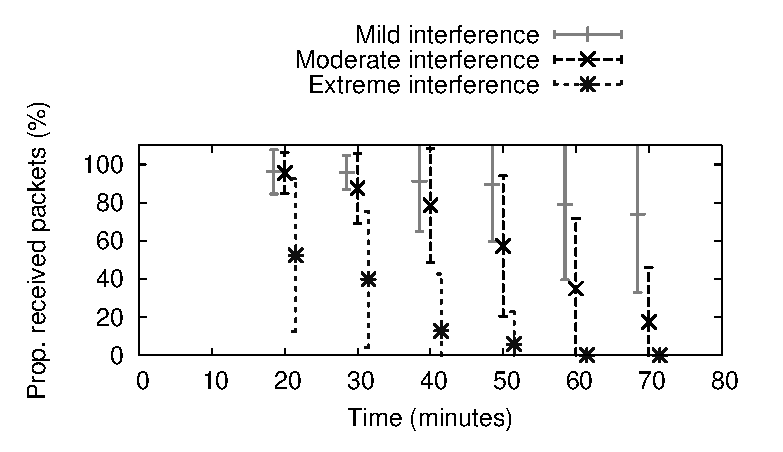
\includegraphics[width=0.45\textwidth]{experiments/single_channel.eps}
\caption{Level of packet loss for mild, moderate and extreme interference levels using single channel}
%\subfigure[Mild Interference]{\label{fig:mild}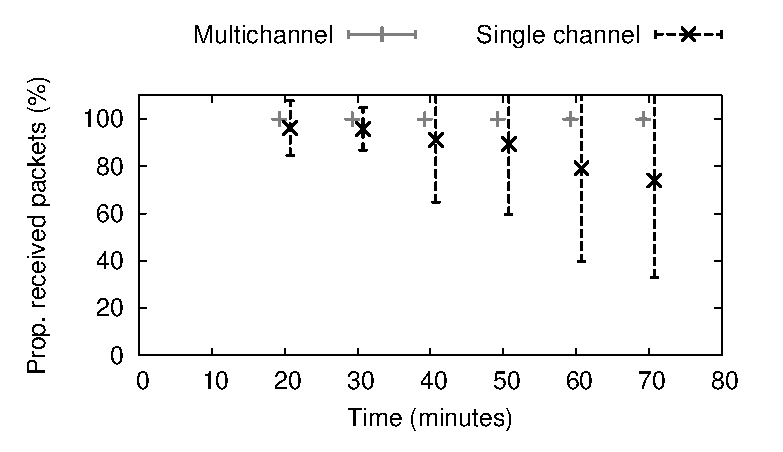
\includegraphics[width=0.45\textwidth]{experiments/mild.eps}}                
%\subfigure[Moderate Interference]{\label{fig:mod}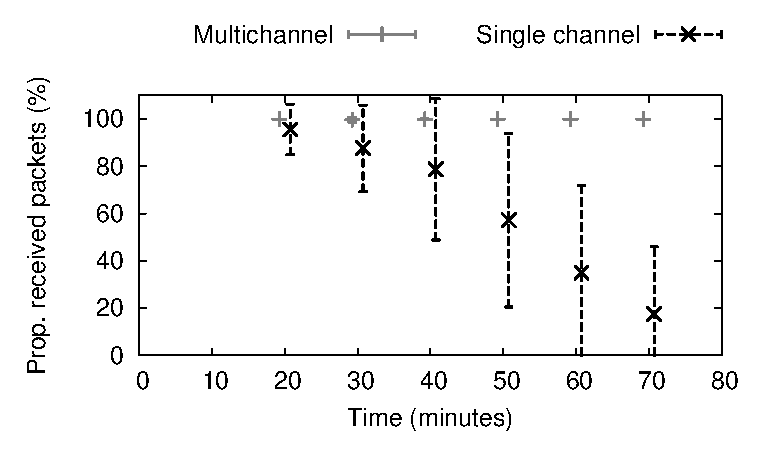
\includegraphics[width=0.45\textwidth]{experiments/moderate.eps}}
%\subfigure[Extreme Interference]{\label{fig:extreme}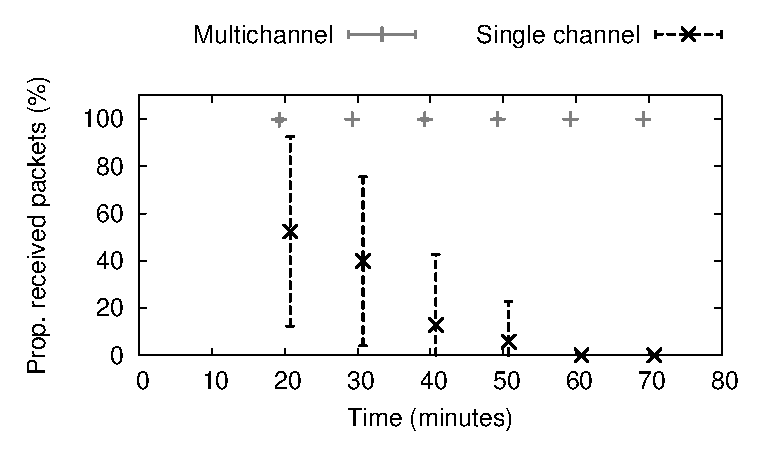
\includegraphics[width=0.45\textwidth]{experiments/extreme.eps}}
%\caption{Level of packet loss for mild, moderate and extreme interference levels using single and multi-channel}
\label{fig:interference}
\end{figure}

\begin{figure}
\centering
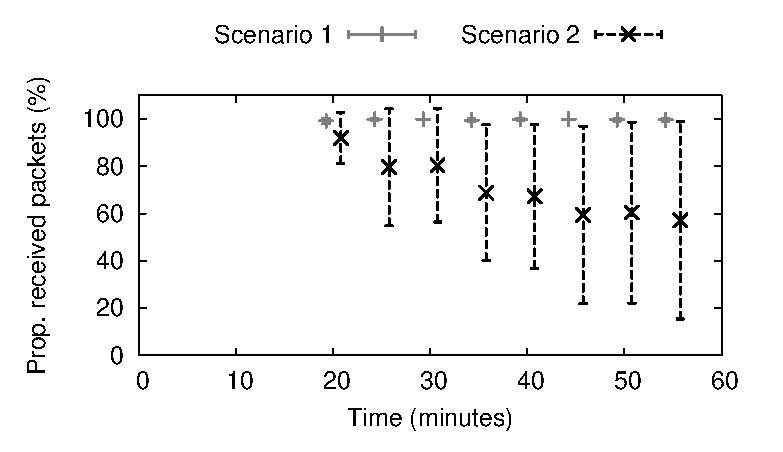
\includegraphics[width=0.45\textwidth]{experiments/multi_channel.eps}
\caption{Level of packet loss for scenario 1 and scenario 2 using multi channel}
\label{fig:multi_interference}
\end{figure}

Figure \ref{fig:interference} shows the results for the original RPL protocol.
It can be seen that the level of packet loss varies considerably between experiments
(the error bars are always large).  It can also be seen that even for mild 
interference there is considerable loss and this gets worse as time proceeds.
In the extreme interference case the loss always goes up until no packets are received.
For mild interference the system evolves until it is losing around 20\% of
packets but this can increase.

For our new multiple channel protocol we consider two interference scenarios.
In scenario 1 half the channels (including the original channel) have no
interference at all and half the channels have extreme interference.
In scenario 2, four channels (including the orginal channel) have no
interference, four have mild, four moderate and four extreme interference.
Figure \ref{fig:multi_interference} shows multi channel results for these
two scenarios.  In scenario 1 the protocol performs extremely well, the packet
loss is near zero and the protocol successfully detects channels with interference.
Scenario 2 has worse results but the protocol still does well at reducing the
effects of interference.  In this case the final result is somewhere between
the mild and the moderate interference level of the single channel case
showing that the protocol has picked some of the channels with the least interference.
The variance in the results is, as with the single channel case, high.  The worst
results happen when channels with interference are picked as those near the
LBPR (which bear the most traffic).   


\subsection{Setup Overhead}
%//overhead?
%trickle - doubled each time but wait for a while so that it won't (affect?) with our protocol (sending messages; need to change channel which might be a problem?)

%//mention how much overhead there is agains RPL. 

%//say it is a one-off and compare it with data transmitted in one hour. packet transmitted high, overhead is negligible - real world, for low bit rate i.e video run for hours/months. "The.. is much smaller compared to the data period and during the data period the nodes can transmit multiple packets to do normal transmission"

%//mention that our protocol can transmit during the set up phase. so rpl set up forms the network then our protocol improves the network at a small cost in terms of messages and while leaving the network functional.

Obviously the system of changing channels and probing to see if a channel is free of interference introduces a certain amount of overhead into
the protocol.  This takes the form of (a) extra messages passed and (b) extra time taken to set up.  Default RPL on ContikiMAC for the topology considered in these experiments completed its set up using 276 packets.  Our multi-channel protocol completed its set up in 716 packets, that is an overhead of 440 packets on top of RPL. 
This overhead comes from the channel changing messages to nodes and neighbours, probing messages, channel confirmation messages and acknowledgement packets which are required to ensure a thorough channel change decision.
However, it is worth mentioning that this is a one-off cost.  This represents (in this experimental set up) approximately one hour of extra packets in the situation of a deployment that is meant to work for weeks or months.  In terms of set up time, our protocol begins to change channels only when the RPL set up process is complete (or at least stablises).  The set up time is 435 seconds beyond the 
RPL set up time of 286 seconds.  However, it should be noted that, in fact, our system remains fully functional and capable of sending packets during
the set up so this set up overhead does not matter to data transmission.
